\section{Logická funkce, její vyjádření pomocí tabulky, algebraického výrazu a map. Úplný součtový a součinový tvar algebraického vyjádření logické funkce. Metody a principy minimalizace logických funkcí. Úprava logické funkce pro realizaci pomocí členů NAND a NOR.}

\subsection{Logická funkce}
Matematický model logického kombinačního obvodu. \\
Jestliže hodnota výroku y závisí na hodnotách výroku \(x1, x2,..,xn\), pak říkáme, že logická proměnná y je logickou funkcí proměnných \(x_1,x_2,..,x_n\). Kde \(x_1,x_2,..,x_n\) je n-tice tvořená prvky 0 a 1.\\

Počet možných logických funkcí je \(2^n\), kde n je počet proměnných.

\begin{figure}[h!]
    \centering
    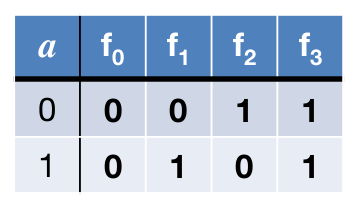
\includegraphics[scale = 0.5]{img/LogFce1.png}
    \caption*{Logická fce jedné proměnné}
\end{figure}

Úplně zadaná logická funkce, je taková funkce kde známe hodnotu pro všechny možné kombinace vstupních hodnot.\\
Neúplně zadaná logická funkce je taková, kde pro některé kombinace vstupních hodnot neznáme hodnota logické funkce. Pro neurčené stavy volíme hodnoty tak aby byla technická realizace co nejjednodušší.\\

\subsubsection*{Vyjádření pravidvostní tabulkou}
Jednotlivé kombinace jsou uspořádány tak, jak roste binární číslo. Řádky tabulky značíme stavovými indexy s.
\begin{figure}
    \centering
    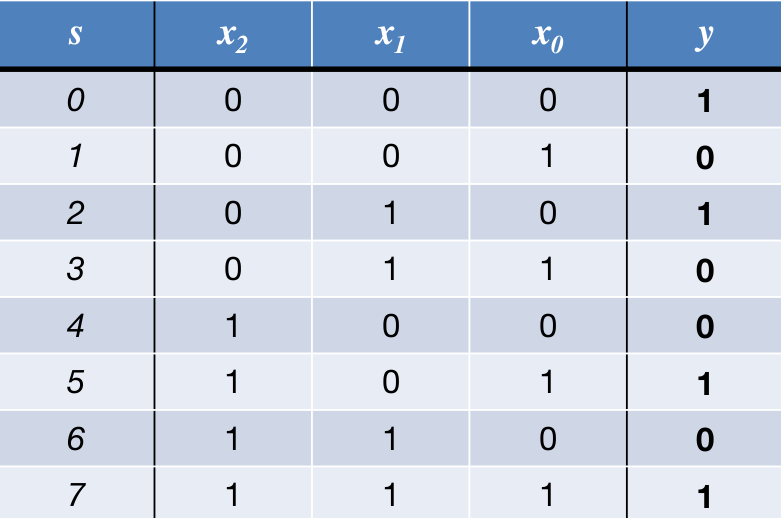
\includegraphics[scale = 0.4]{img/PravTabulka.png}
\end{figure}

\subsubsection*{Vyjádření pomocí algebraického výrazu}
Logický výraz je tvořen logickými proměnnými a operátory.\\
Soustava operátorů musí být volena tak, aby umožnila vyjádřit libovolně složitou funkci. Tato soustava se nazývá úplný soubor logických funkcí. \\
Úplné soubory:
\begin{enumerate}
    \item AND, OR, NOT
    \item AND, XOR, XNOR
    \item Implikace, XOR
    \item Shefferova funkce(NAND)
    \item Piercova funkce(NOR)
\end{enumerate}

\subsubsection*{Vyjádření pomocí map}
Karnaughovy mapy.\\
Uspořádány do čtverce nebo obdélníka. Každému poli jednoznačně odpovídá jedna kombinace vstupních proměnných. \\
Dovnitř do pole zapisujeme hodnotu výstupní proměnné.\\
Sousední pole jsou ta, která se dotýkají, pole na okrajích mapy(konce řádků, sloupců, rohy mapy), u mapy pro 5 a 6 proměnných pole symetrická podle os(vodorovné, svislé).\\
Sousední pole odpovídají mintermům či maxtermům, které se liší pouze v jedné hodnotě vstupní proměnné.\\
\subsubsection*{Tvorba map}
Vzniká zrcadlením. \\
Při jednom vodorovném/svislém kroku mapou se změní vždy jedna hodnota vstupní proměnné(Grayův kód).\\
Názorná je do 4 proměnných. \\
\newpage
\begin{figure}[h!]
    \centering
    \begin{minipage}[b]{0.4\textwidth}
        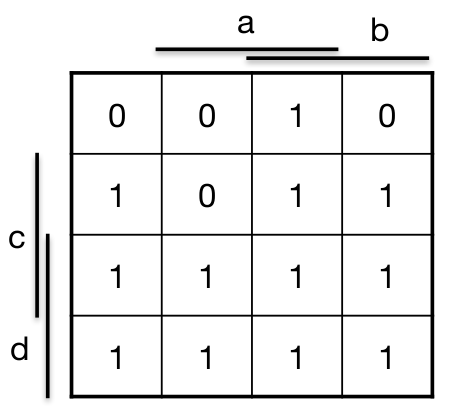
\includegraphics[width=\textwidth]{img/Mapa4.png}
    \end{minipage}
    \hfill
    \begin{minipage}[b]{0.4\textwidth}
        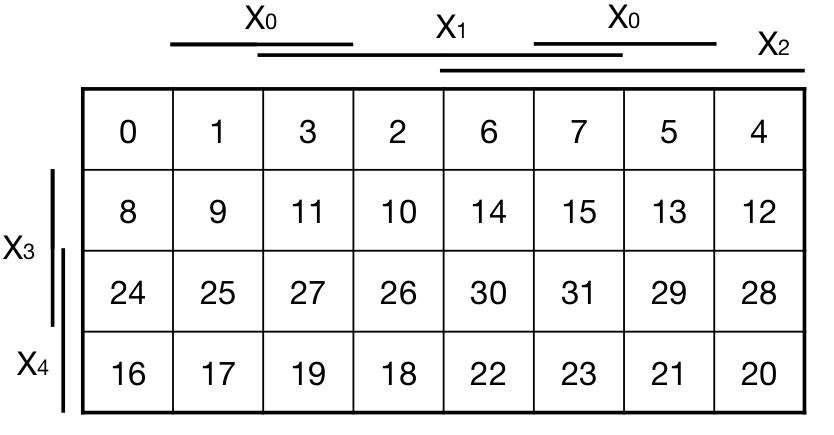
\includegraphics[width=\textwidth]{img/Mapa5.png}
    \end{minipage}
\end{figure}

\subsection*{Úplný součtový a součinový tvar}
Term je výraz tvořený pouze proměnnými a operacemi AND(konjukce) nebo OR (disjunkce).\\
Minterm obsahuje všechny proměnné a pouze operaci AND.\\
Maxterm obsahuje všechny proměnné a pouze operaci OR.
\begin{center}
    Minterm: \(y = (x_2 \cdot \overline{x_1} \cdot x_0)\)\\
    Maxterm: \(y = (\overline{x_2} \cdot x_1 \cdot \overline{x_0})\)
\end{center}

Logickou funkci lze zapsat ve dvou základních tvarech.\\
\begin{itemize}
    \item Součtový tvar - úplná disjnukční normální forma. Součet mintermů, pro které funkce nabývá hodnotu 1.
    \item Součinový tvar - úplná konjunktní normální forma. Součin maxtermů, pro které funkce nabývá hodnotu 0.
\end{itemize}

\subsubsection*{Součtový tvar - ÚDNF}
Součet elementárních logických funkcí, z nichž každá má hodnotu 1 pouze pro jeden řádek tabulky - takové funkce jsou mintermy.\\
V mintermu zapisujeme proměnné, které nabývají v příslušné kombinaci hodnoty 1 jako přímé a proměnné, které nabývají hodnoty 0 jako negované.\\
Minterm musí obsahovat všechny proměnné funkce.\\

\subsubsection*{Součinový tvar - ÚKNF}
Součin elementárních logických funkcí, z nichž každá má hodnotu 0 pouze pro jeden řádek tabulky - takové funkce jsou maxtermy.\\
V maxtermu zapisujeme proměnné přesně naopak oproti mintermu.\\
Maxterm musí obsahovat všechny proměnné funkce.\\
\newpage
\begin{figure}
    \centering
    \includegraphics*[scale = 0.4]{img/Tvary.png}
\end{figure}
Rovnice pak jsou:
\begin{center}
    ÚDNF: \(y=\sum_{n = 1}(0,2,5,7)= \overline{x_2} \cdot \overline{x_1} \cdot \overline{x_0} + \overline{x_2} \cdot x_1 \cdot \overline{x_0} + x_2 \cdot \overline{x_1} \cdot x_0 + x_2 \cdot x_1 \cdot x_0 \)\\
    ÚKNF: \(y = \prod (1,3,4,6) = (x_2 \cdot x_1 \cdot \overline{x_0}) + (x_2 \cdot \overline{x_1} \cdot \overline{x_0}) + (\overline{x_2} \cdot x_1 \cdot x_0) + (\overline{x_2} \cdot \overline{x_1} \cdot x_0)\)
\end{center}
\subsection{Minimalizace logické funkce}
Vyjádření logické funce považujeme za minimální pokud má minimální počet termů, minimální počet nezávisle proměnných v každném termu, minimální počet negovaných proměnných.\\
Metody minimalizace jsou pomocí algebraických výrazů, pomocí map, speciálními metodami(např. metoda Quine-McCluskey).\\
\subsubsection*{Minimalizace pomocí algebraických výrazů}
Pro součtový tvar to je spojování mintermů tak aby se vyloučily proměnné (\(a \cdot \overline{b} + b \cdot a = a(\overline{b} + b) = a\)). Vyloučením proměnných vznikají implikanty. Implikant považujeme za větší pokud pokrývá větší počet bodů funkce(tvořen menším počtem proměnných). Výsledkem je minimální disjunktní normální forma - MDNF.\\
Pro součinový tvar spojování maxtermů tak aby se vyloučily proměnné(\((a+b)\cdot(a+\overline{b}) = a + (b \cdot \overline{b}) = a\)).Vyloučením proměnných vznikají inhibenty. Výsledkem je minimální konjunktní normální forma. \\
Jak MDNF tak MKNF může mít jedna funkce více než jednu.

\subsubsection*{Minimalizace Karnaughovy mapy}
Princip spočívá vpokrytí všech 1 (případně 0) soustavou smyček, přičemž:
\begin{itemize}
    \item Sousední pole se stejnou výstupní hodnotou lze spojovat do větších smyček.
    \item Smyčky musí být co největší, ale vždy obsahovat \(2^i\) polí.
    \item Smyček musí být co nejmenší počet
    \item Neurčené stavy nahrazujem čísly tak, abychom dostali co největší smyčky
\end{itemize}

\begin{figure}
    \centering
    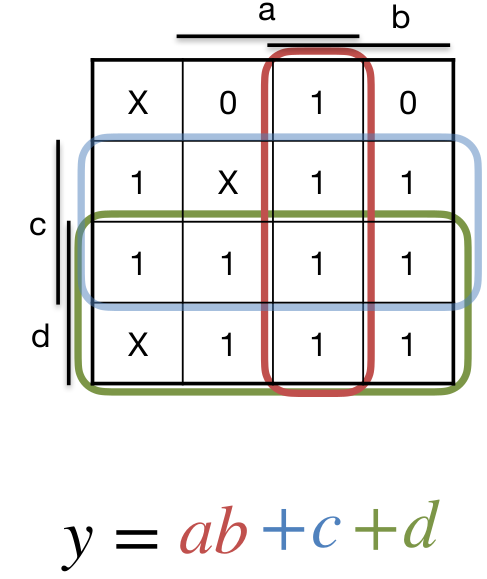
\includegraphics[scale = 0.3]{img/minMapa.png}
\end{figure}

\subsection{Úprava logické funkce pro realizaci pomocí NAND a NOR}
Pro nejjednodušší technickou realizaci je vhodné mít co nejmíň funkcí v úplném souboru. Existují 2 minimální soubory, NAND a NOR.
\subsubsection*{Úprava na členy NAND}
Při úpravách na NAND vyjdeme ze součtové formy a použijeme DeMorganův zákon. \(\overline{a+b} = \overline{a} \cdot \overline{b}\)
Příklad úpravy na NAND:
\begin{center}
    \(\overline{x_1} \cdot \overline{x_0} + x_1 \cdot x_0 = \overline{\overline{\overline{x_1}\cdot\overline{x_0} + x_1 \cdot x_0}} = \overline{\overline{\overline{x_1}\cdot \overline{x_0}}\cdot\overline{x_1 \cdot x_0}}\)
\end{center}
\subsubsection*{Úprava na členy NOR}
Při úpravách vycházíme ze součinové formy a použijeme DeMorganův zákon. \(\overline{a \cdot b} = \overline{a} + \overline{b}\)
Příklad úpravy na NOR:
\begin{center}
    \((\overline{x_1}+\overline{x_0})\cdot (x_1 + x_0) = \overline{\overline{(\overline{x_1}+\overline{x_0})\cdot (x_1 + x_0)}} = \overline{\overline{(\overline{x_1}+\overline{x_0})}+\overline{(x_1+x_0)}}\)
\end{center}
\section{Přechodné děje v kombinačních logických obvodech, hazardní stavy (souběhový, dynamický a statický hazard), metody detekce a řešení statického hazardu ve dvoustupňové struktuře NAND-NAND, konsensus, řešení hazardu pomocí sekvenčních obvodů.}


\section{Rozdíl mezi kombinačním a sekvenčním logickým obvodem. Klopné obvody: RS, D, JK, T, hladinové, hranové a master-slave, pravdivostní tabulka, pojem metastabilita v sekvenčních logických obvodech.}


\section{Kombinační logické obvody: binární dekodér, multiplexor, demultiplexor, kodér, prioritní kodér, číslicový komparátor, binární sčítačka a odčítačka. Druhý doplněk. Logické obvody s třístavovým výstupem a s otevřeným kolektorem. Připojování zařízení na sběrnici.}

\section{Sekvenční logické obvody: posuvný registr, posuvné registry se zpětnou vazbou (kruhový čítač, Johnsonův čítač, lineární čítač - LFSR), asynchronní a synchronní čítače, popis jejich funkce pomocí jazyka HDL. Vysvětlete pojmy HDL jazyka: souběžný a sekvenční příkaz, okamžité a odložené přiřazení.}


\section{Konečné stavové automaty: Obecný (Huffmanův) model sekvenčního logického obvodu, přechodová funkce, výstupní funkce, budicí funkce. Mealyho, Mooreho a autonomní automat. Popis konečného automatu pomocí stavového diagramu, tabulky přechodů a tabulky výstupů. Návrhová tabulka (budicí funkce KO).}

